\section{Theory}
\label{sec:theory}
This section aims to summarize the basic principles that underpin the operation of diode lasers.

\subsection{The Diode Laser}
\label{sec:diodelaser}
The term 'laser' stands for \textbf{L}ight \textbf{A}mplification by \textbf{S}timulated \textbf{E}mission of
\textbf{R}adiation. A laser is a unique source of electromagnetic radiation, characterized by
properties such as an extensive coherence length, monochromaticity, and concentrated intensity
paired with minimal divergence. Owing to these distinctive features, lasers are versatile and find
applications in various areas. Within this experiment, we employ a diode laser as a tool
for spectroscopic analysis.\\
\noindent
The operation of a laser amplifies radiation by the mechanism of stimulated emission. For a laser to function
effectively, stimulated emission must dominate over both absorption and spontaneous emission within the laser medium.
This is achieved through establishing population inversion. Additionally, an optical resonator is used to enhance the
emitted radiation further. \\
\\
\noindent
The laser device used in this experiment has at its core a semiconducting diode. It consists of at least three layers:
the active layer, the n-doped layer and the p-doped layer. In the n- and p-doped layer, free charge carriers in the
form of electrons and electron holes respectively, are present. The active layer of the laser diode forms a cavity. A
injection current is run through the diode, causing
the electrons and electron holes to recombinate in the active layer between the n- and p-doted layers.
Therefore, the wavelength of the emitted photons corresponds to the width of the band gap of the semiconductors
material. This process can also be caused by another photon; this process is called stimulated emission.
If the injection current is high enough, the amplification through stimulated emission exceeds the optical
losses in the diode and population inversion can be achieved. In this case, the diode emits a coherent beam.
The emitted radiation is confined by refraction to a channel inside the diode (the active layer), with facets at the
ends of the channel that serve as cavity mirrors and output couplers. The diode used in this experiment emits most
radiation through the front facet, as the back facet is for the most part reflective. A schematic display of such a
laser diode chip is given in Figure~\ref{fig:diode}.
\begin{figure}[H]
  \centering
  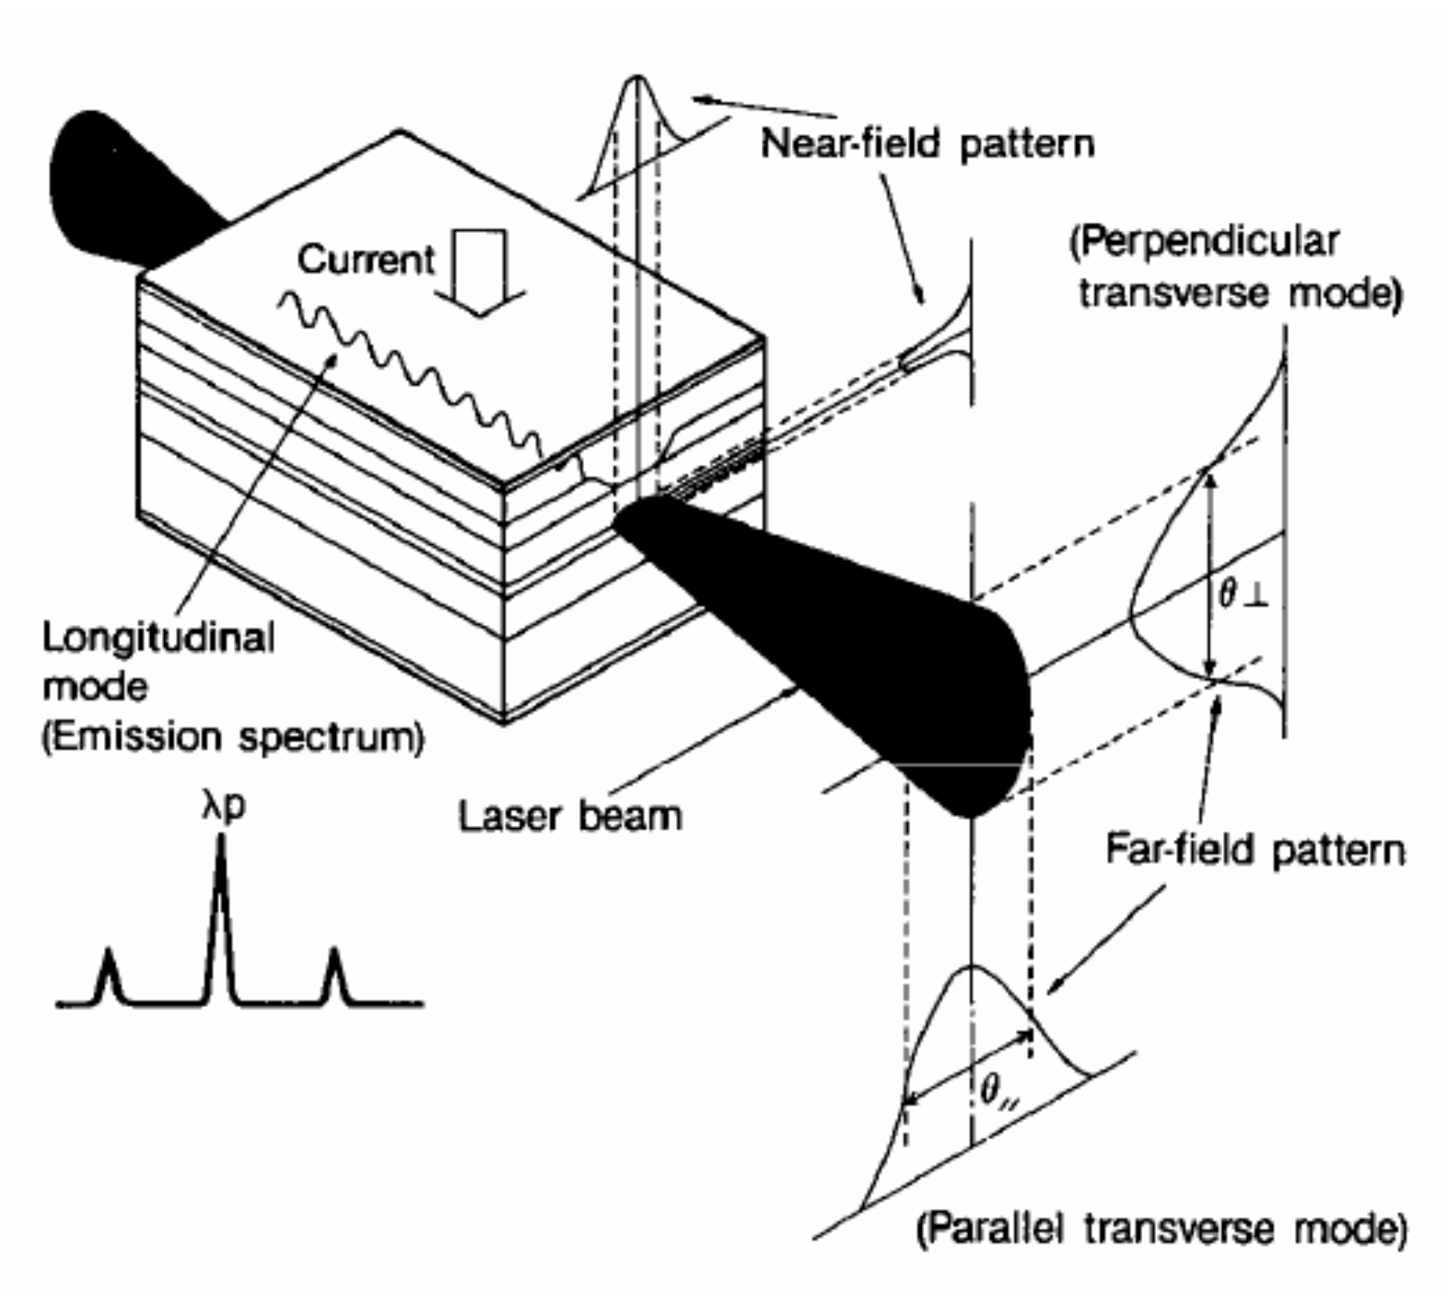
\includegraphics[scale=0.4]{./pictures/Diode-schematisch.png}
 \caption{Schematic display of a laser diode (LD) chip~\cite{teachspin}.}
 \label{fig:diode}
\end{figure}
\noindent
However, the light emitted by the raw laser diode chip has certain limitations; the beam is strongly diverging,
the frequency stability is very sensitive to optical feedback and the radiation has a linewidth of $~10$ times the
linewidth of atomic transitions. To overcome these problems, a configuration like the one displayed in
Figure~\ref{fig:laser-system} can be employed.
\begin{figure}
  \centering
  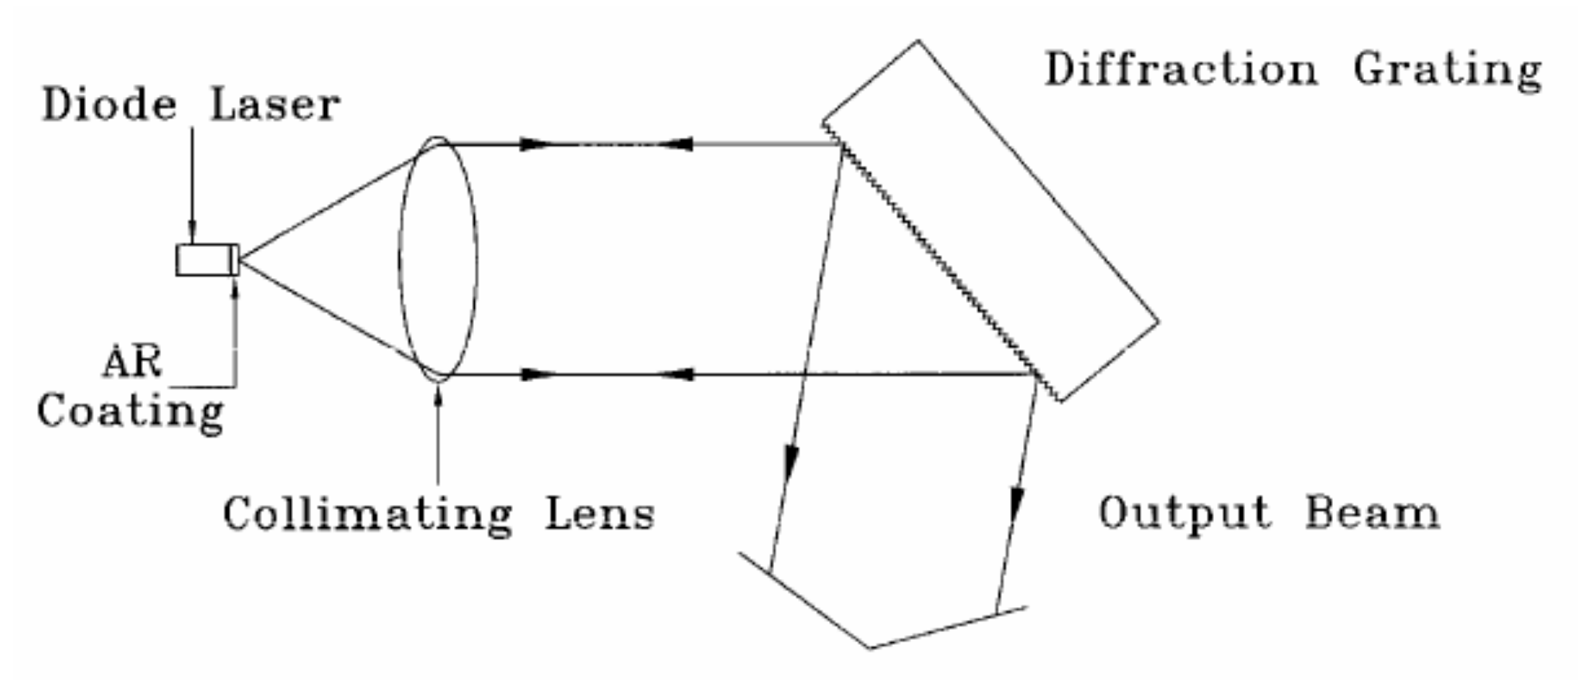
\includegraphics[scale=0.4]{./pictures/Laser-system.png}
  \caption{Configuration of a laser system~\cite{teachspin}.}
  \label{fig:laser-system}
\end{figure}
\noindent
Here, a collimating lens is used to prevent the divergence of the laser beam. To improve frequency stability,
around $\SI{15}{\percent}$ of light is routed back into the diode through the use of a diffraction grating.
This grating acts as an external cavity (in addition to the internal cavity inside the laser diode chip).
The grating also reduces the linewidth of the laser beam to less than $\nu = \SI{1}{\mega\hertz}$, which is
smaller than the atomic transitions linewidths.

\subsection{Tuning of the Diode Laser}
\label{sec:tuning}
After the lasing process has started, the beam mostly consists of light with the frequency that offers the highest
net optical gain. The exact frequency depends on several factors, which are displayed in
Figure~\ref{fig:diode-frequency}.
